\documentclass[prl,showpacs,superscriptaddress,twocolumn,longbibliography]{revtex4-1}

\usepackage{hyperref}
\usepackage{url}
\usepackage{color}
\usepackage[usenames,dvipsnames]{xcolor}
\usepackage{amsmath,amsthm,amssymb}
\usepackage{graphicx}
\usepackage{float}
\usepackage{epsfig}
\usepackage{bm}% bold math
\usepackage{mathrsfs}
\usepackage{multirow}
\usepackage[all]{xy} 
\usepackage{pbox}
\usepackage{verbatim}
\usepackage{braket}
\usepackage{mathtools}
\usepackage{bm}
\usepackage{tikz}
\usepackage{xcolor}
\newcommand{\red}[1]{\textcolor{red}{#1}} 
\usepackage{mathtools}
\newcommand{\change}[1]{\textcolor{blue}{#1}}
\usepackage{mathtools}
%\usepackage{tabstackengine}
\usepackage{enumerate}   


\begin{document}

\author{Erin Aho}
\author{Albert Nyarko-Agyei}
\author{Soham Talukdar}

\title{Identifying an optimal feature set to analyse species richness in Butterflies}


\begin{abstract}
Butterflies are important taxa, both ecologically and culturally, but have been declining in population despite conservation efforts. To improve understanding of where to focus conservation efforts we aim to identify which features are the most informative in terms of species richness in an area.
The species count of butterflies in 45 broad regions was analysed. Based on existing research, we decided on a set of 28 features, both bioclimatic and anthropogenic, which are known to affect species richness. We generated a dataset by taking the mean across our regions for each feature, using open-source GIS tools. After researching current feature selection methods, we decided to use Joint Mutual Information (JMI) as our selection criterion, due to the high amount of mutual information in many of our features, and the strong performance JMI has been shown to have form small data samples. After performing feature selection on our dataset using JMI, we were able to identify that the most informative set of 5 features is Annual Precipitation, Isothermality, Mean Diurnal Temperature Range, Precipitation of the Warmest Quarter, and the Percent of Urbanization. We discuss possible limitations of our approach, and areas further research is needed in order to better understand butterfly species richness.
\end{abstract}

\maketitle

\noindent {\bf\em Introduction.--}
Butterflies (suborder Rhopalocera) of the order Lepidoptera is one of the most widespread and widely known insect orders with maybe more than 350,000 species worldwide. Approximately 160,000 species have been described, about 20,000 of which are from Africa\cite{Arnold}. Butterflies have had a significant impact on western culture since the ancient Greeks. They were a metaphorical resemblance to the soul and was depicted symbolically in painting and religious texts throughout history\cite{Dicke2000}. Hence the impact of butterflies transcendents beyond ecological importance.

Over the years, conservation efforts focussed on protecting rare, charismatic, and endangered species. However, current reports mention a steep loss in the number of formerly abundant butterfly populations along with other insect taxa \cite{Wagner2021}. Important aspects of the insect decline phenomenon remain largely unknown. With so little data from outside Europe, it is difficult to gauge how widespread the phenomenon is, especially in the tropics and southern temperate regions, where more than 85\% of all insect species occur. Many studies show that net loss of insect abundance/biomass has not been reported from all study locations and multiple challenges are faced when trying to answer questions regarding the magnitude and reason for insect decline \cite{Montgomery2020}.

\noindent {\bf Existing understanding:}

The richness and viability of any species depend upon several natural and human-induced factors. Butterflies act as a bioindicator of environmental damage and a useful indicator of urbanization because they are readily surveyed to changes in microclimate, temperature and solar radiation\cite{Clark2007}.Changes in the dry or wet climate cause a shift in microclimate, resulting in a difference in rainfall and average temperature affecting the population of several species of butterflies\cite{Haneda2019}. Current ecological research increasingly addresses issues related to habitat fragmentation, global environmental change and loss of biodiversity. Against this background, understanding the relationship between species richness and the area is particularly important. Connor \& McCoy (1979) also discussed the two major hypotheses explaining why richness should increase with area:(i) the environmental heterogeneity (habitat diversity)hypothesis; and (ii) the demographic process hypothesis. The first explanation is a pattern-based view of SAR(species-area relationships), such that larger areas have a higher probability of containing more habitat types; this increase of habitat diversity with area generates the SAR because of species' habitat associations.In contrast, the demographic explanation is process-based, incorporating the dynamic processes of dispersal, colonization, speciation and extinction at multiple spatial scales. Larger areas have higher probabilities of colonization and speciation and lower probabilities of extinction, fostering higher diversity\cite{Drakare2006}. Several studies confirm that agricultural land use harms the semi-natural grassland and can affect both habitat suitability and availability of any individual species related to grasslands\cite{smith}. Urbanization is one of the most important causes of natural ecosystem loss and habitat fragmentation including decreased plant species diversity, reduced water quality, and increased air and soil pollution triggering species diversity decline\cite{smith,Tzortzakaki2019}. Species richness (i.e., the number of species occurring in a given area) is commonly used as an integrative descriptor of the community, as it is influenced by a large number of environmental factors such as environmental stability, ecosystem productivity and heterogeneity, and biological factorsstep\cite{Park2003}.

We aim to help shrink this gap in information by finding which features are the most important to track, and what features impact their species density the most so that we can better understand how the impacts of climate change and further anthropogenic habitat disruption will affect butterflies moving forward. We have thus created a set of features based on the factors which are important to biodiversity, and want to find the most relevant/informative features for Butterflies in particular.


\noindent {\bf\em Method.--}
An important step to model implementation is to select the features, that can provide a substantial result based on our requirements. However, a considerable thought process is put into deciding why and which features should be considered. Since our initial data extends over a significant geographical stretch, it becomes necessary to take into the factors of different bioclimatic indicators. These indicators are numerous meteorological variables and/or derived indices that have been formulated, calculated and applied to explain the geographic distribution of natural populations along climate gradients,  characterized by intra-annual patterns of temperature and precipitation. They mainly result from primary - observed or modelled - climate fields (e.g. minimum, maximum and  mean  temperature,  precipitation  amount)  and  contribute  to  delineate  the  bioclimatic  “envelope” for species in terms of favourable environmental conditions, also referred to as "suitability"\cite{Noce2020}. 

Based on the U.S. Geological Survey (USGS) there are 35 such bioindicators, out of which only 19 common indicators are selected. To analyse the spatial data for different bioclimatic indicators, we gathered the vector and raster layers from various data centres for the area required for our work and used QGIS software to get a visual understanding of it\cite{a1,b2,c3,d4,e5,f6,g7,h8}.
Ecologists or conservation biologists are interested in species density, for some particular amount of area, in its own right. Because species density is so sensitive to area (and, ultimately, to the number of individuals observed or collected), it is useful to decompose it into the product of two quantities: species richness (number of species represented by some particular number, N, of individuals) and total individual density (number of individuals N, disregarding species, in some particular amount of area A):
\[
    \left(\frac{Species}{Area}\right) =  \left(\frac{Species}{N individual}\right) \times \left(\frac{N individual}{Area}\right)
\]
This decomposition demonstrates that the number of species per sampling unit
reflects both the underlying species richness and
the total number of individuals sampled\cite{Brose2003}.
The reason for the use of feature selection over PCA is to have easily interpretable features which can be readily used for analysis. Decided to use a filter method, not a wrapper method, to limit risk of overfitting and the risk of it is quiet large due to small number of observations compared to number of features.
Choosing a criterion is not trivial and decades of theoretical and heuristic approaches have produced a large number of options. A study provided a unified framework of many popular criterion, comparing their performances and theoretical bases. The study found that We note that JMI, (which both balances the relevancy and redundancy terms and includes the conditional redundancy) outperforms all other criteria\cite{Brown2012}. Based on this, we chose to implement a JMI based criterion.
Battiti (1994) presents the Mutual Information Feature Selection (MIFS) criterion:

\[ 
    J_{mifs}(X_k) = I(X_k;Y) - \beta \sum_{X_j\in S} I(X_k;X_j)
\]

S is the set of currently selected features.The $ \beta $ in the MIFS criterion is a configurable parameter, which must be set experimentally. Using $\beta  = 0 $ would be equivalent to $J_{mim}(X_k)$, selecting features independently, while a larger value will place more emphasis on reducing inter-feature dependencies. In experiments, Battiti found that $\beta  = 1$ is often optimal, though with no strong theory to explain why. The MIFS criterion focuses on reducing redundancy; an alternative approach was proposed by Yang and Moody (1999), and also later by Meyer et al. (2008) using the Joint Mutual Information (JMI), to focus on increasing complementary information between features\cite{Brown2012}. The JMI score for feature $X_k$ is:
\[ 
    J_{jmi}(X_k) =  \sum_{X_j\in S} I(X_kX_j;Y)
\]
However, there are problems that aises from mutual information based feature selection. One such is that although it is simple to compute entropy and consequently mutual information for discrete random variables, most of the time we have continuous measurements in real life datasets. Rounding them to the nearest integer, might seem tempting but it introduces a bias into our MI estimates. To counteract the problem used the well established kNN based MI estimation methods in the case when both X and y are continuous\cite{Daniel,Ross2014}. We used the sklearn based Python implementation on Github\cite{i9}.


\noindent {\bf\em Results.--}
\begin{center}
\begin{tabular}{||c c||} 
 \hline
Top 6 Features & MI \\
 \hline\hline
 Mean annual precipitation & 0.516\\ 
 \hline
 Mean isothermality & 0.652\\
  \hline
 Elevation & 0.539\\
 \hline
 Mean Diurnal Range & 0.507\\
 \hline
 Precipitation of warmest quarter & 0.499\\
 \hline
 Mean min temp of coldest month & 0.457\\ [1ex] 
 \hline
\end{tabular}
\end{center}

The result of the JMI feature selection algorithm highlighted a set of features that have high mutual information with the target variable of this paper, species density. The mean annual precipitation was the first feature selected by the algorithm. This means that when we took each feature and the target variable, this feature had the highest amount of information gain. The next selected feature was also annual measures of the respective variables, potentially signifying the versatility of the mean of over this timeframe to persevering information. There were significant falls in information gain after the addition of the 7th and the 24th variables meaning that the dataset was already saturated with information and the addition of these variables had started to skew our information on the target variable rather than keep our knowledge uniform because this would be associated with high levels of entropy and mutual information.

\begin{center}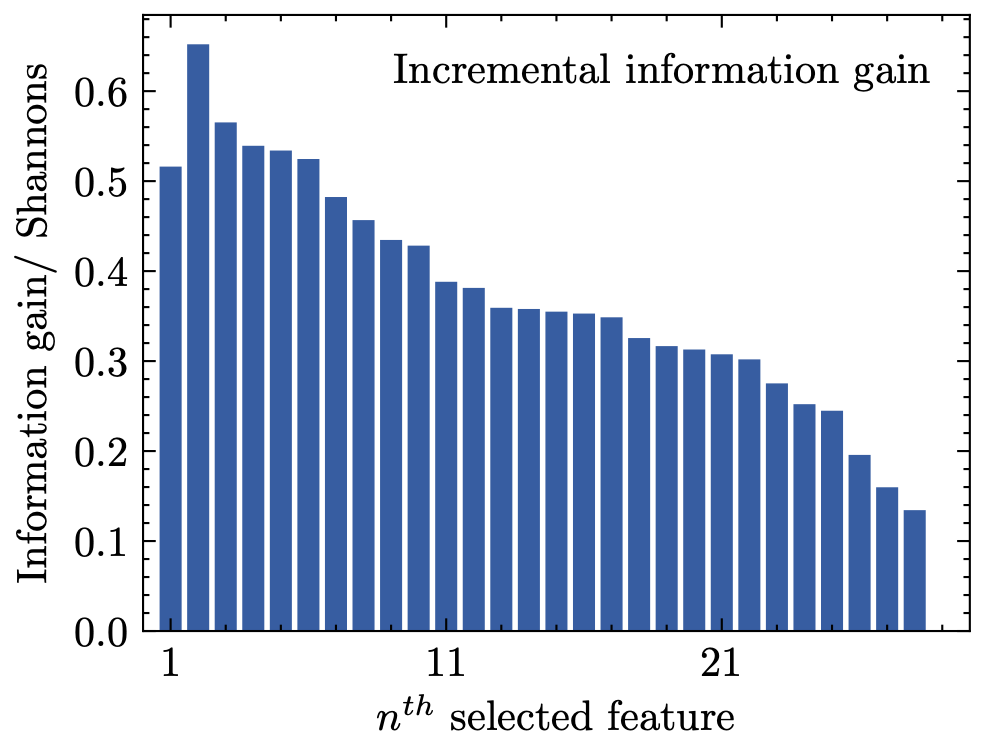
\includegraphics[width=240pt]{Features.png}\end{center}


\noindent {\bf\em Discussion.--}
From the figure, we can see that the highest information gain to the set of selected features was after adding the mean isothermality and there is scientific material that supports this idea of isothermality being one of the crucial factors to species richness \cite{rueda-m_environmental_2021}. Subsequently selected feature still added information however the resulting information gain was strictly decreasing. This is natural if information is being repeated across variables so by the addition of the 23rd variable, the complexity of the distribution of butterflies has already been captured by the selected variables hence the low information gain from new features. 
\newline
\newline
It is interesting to consider the correlation of the variables and the species density along with their order of selection. From the original list of features, the mean minimum temp of the coldest month had the highest correlation with the species density at 0.572 but it was only the 6th selected feature. The next highest correlated feature was mean annual precipitation and this was the first feature to be selected by the JMI algorithm. Interestingly the mean temperature annual range and the precipitation in the wettest quarter were the 3rd and 4th highest in terms of the correlation however they were one of the last features to be selected. Theoretically, this supports the idea that features that repeat information are not being selected but rather, the features that increase the information in the features selected so far are prioritised by the method \cite{afshar_dimensionality_2021}. In all, the dataset had seven metrics regarding precipitation in the given region. It is understandable therefore that by the addition of the seventh metric for precipitation, the information in this feature was redundant despite its high correlation with the target variable.
\newline
\newline
A limitation of our method is the concept that for a given area if more time is spent researching butterflies in that area, then it is likely that more species will be found. While butterflies are one of the most studied taxa, there is still likely to be a large knowledge gap, particularly in remote areas. At the very least the robustness of species counting methods such as counts along a transect have been called into question by Kevin Gross et al \cite{gross_robustness_2007}. It is hard to account for this and estimate which features have been helped or diminished by these factors when it comes to the ranking but these are helpful to keep in mind.  
\newline
\newline
One must also consider the flaws of the JMI algorithm. In particular, it takes a greedy approach by selecting the local maxima of groups of features that have the highest mutual information with the target variable but this approach "lacks theoretical guarantees" according to Gao et el \cite{gao_variational_2016}. A further study could implement JMIN which tackles this issue of local maxima by conducting more searches on combinations of features.

\noindent {\bf\em Conclusion.--}

The key takeaway from the study is that the features within our original list of features are highly interdependent and so the absence of one feature can be accounted for by the inclusion of information from other features. This is backed by studies that present conflicting arguments for the level of importance of the island indicator variable\cite{kalmar_unified_2007}. Kalmar and Currie find that most variation in species density is not context-specific, but is dependent more on general environmental constraints such as if the region is an island or not. It must be noted that half of the islands used in their studies had an area between 0.085 and 625km$^2$ and only one of the islands in our dataset fell in this category. This makes the extension of their findings to ours difficult nonetheless it gives context to the difficulty of identifying important features.
\newline
\newline
Overall, we have been successful in reducing the original 28 features to a small subset of informative features for butterfly species richness. We wanted to preserve the interpretability of any features obtained from this study so we rejected PCA and other linear dimension reduction techniques that convolute the meaning of the data in favour of a method that allows for a clearer understanding of the distribution of butterflies. These findings can be used to help identify areas to focus conservation efforts on. However, they highlight that the list of features that affect butterfly richness is complex and that many connections exist between these variables. Lastly, some success has been found in using an embedded feature selection algorithm in conjunction with a learning algorithm. This could be an area to explore further, to create a robust method of picking features while also creating predictions.


\bibliography{Bibliography}
\bibliographystyle{apsrev4-1}

\end{document}